\chapter{ប៉ារ៉ាបូល}
\section{សញ្ញាណប៉ារ៉ាបូល}
%
\begin{definition}
	\emph{ប៉ារ៉ាបូល} ជាសំណុំចំណុចនៅក្នុងប្លង់ដែលមានចម្ងាយស្មើពីចំណុចនឹងមួយ និង បន្ទាត់នឹងមួយ។
\end{definition}
%
\begin{figure}[H]
	\centering
	\caption{ប៉ារ៉ាបូល}
	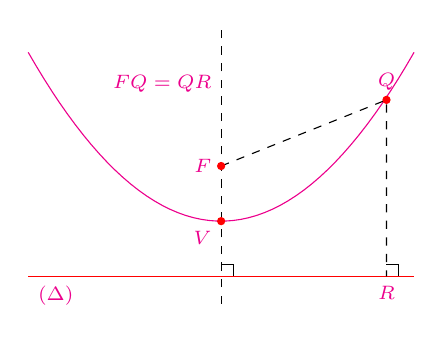
\begin{tikzpicture}[x=.7cm,y=.7cm,every node/.style={font=\scriptsize,text=magenta}]
	\coordinate(O)at(0,0);
	\coordinate(V)at(O);
	\coordinate(X')at(-3.5,0);
	\coordinate(X)at(3.5,0);
	\coordinate(Y')at(0,-1.5);
	\coordinate(Y)at(0,3.5);
	\coordinate(V)at(O);
	\coordinate(F)at(0,1);
	\coordinate(D)at(0,-1);
	\coordinate(Q)at(3,2.2);
	\coordinate(R)at(Q|-D);
	\draw([yshift=1ex]D)--([xshift=1ex,yshift=1ex]D)--([xshift=1ex]D);
	\draw[magenta]plot[samples=50,domain=-3.5:3.5](\x,{.25*\x*\x});
	\draw[red](D-|X')node[below right]{$ (\Delta) $}--(D-|X);
	\draw[dashed](F)node[left]{$ F $}--(Q)node[above]{$ Q $}--(R)node[below]{$ R $};
	\draw[dashed](Y')--(Y);
	\draw([yshift=1ex]R)--([xshift=1ex,yshift=1ex]R)--([xshift=1ex]R);
	\foreach\p in{V,F,Q}{\fill[red](\p)circle(1.5pt);}
	\node[below left]at(V){$ V $};
	\node[left] at(0,2.5){$ FQ=QR $};
  \tkzMarkSegments[mark=||,color=blue](F,Q Q,R)
	\end{tikzpicture}
\end{figure}
%
\begin{itemize}
	\item ជាទូទៅប៉ារ៉ាបូលតាងដោយ $ (P) $
	\item ចំណុចនឹងនោះហៅថា​ \emph{កំណុំ} តាងដោយ $ F $
	\item បន្ទាត់នឹងនោះហៅថា​ \emph{បន្ទាត់ប្រាប់ទិស} តាងដោយ $ (\Delta) $
	\item បន្ទាត់ដែលកាត់តាមកំណុំហើយកែងនឹងបន្ទាត់ប្រាប់ទិសជា \emph{អ័ក្សឆ្លុះ}
	\item ប្រសព្វរវាង បន្ទាត់ប្រាប់ទិស និង អ័ក្សឆ្លុះ ហៅថា \emph{កំពូល} តាងដោយ $ V $
	\item បើ $ Q $ ជាចំណុចនៅលើប៉ារ៉ាបូល និង $ R $ ជាចំណោលកែងនៃ $ Q $ លើបន្ទាត់ប្រាប់ទិស នោះយើងបាន $ FQ=QR $~។
\end{itemize}
%
\newpage
\section{របៀបសង់ប៉ារ៉ាបូល}
ហើយតាម $ 2p $ ជាចម្ងាយពីកំណុំ $ F $ ទៅបន្ទាត់ប្រាប់ទិស $ (\Delta) $ ដែល $ p>0 $ ពិនិត្យរូប
\begin{figure}[H]
  \centering
  \begin{tikzpicture}[x=.75cm,y=.75cm,every node/.append style={font=\scriptsize}]
  \coordinate(D')at(-6,-1);
  \coordinate(D)at(6,-1);
  \coordinate(F)at(0,1);
  \draw[color=blue](D')--node[sloped,very near end,below]{$ (\Delta) $}(D);
  \fill[color=black](F)circle(1.25pt)node[above right]{$ F $};
  \end{tikzpicture}
\end{figure}
\noindent
នោះគេអាចសង់ប៉ារ៉ាបូលដែលមានកំណុំ $ F $ និងបន្ទាត់ប្រាប់ទិស $ (\Delta) $ តាមជំហ៊ាន
\begin{enumerate}[k]
  \item គូសអង្កត់ $ FH $ ដែល $ H $ ជាចំណោលកែងនៃ $ F $ លើបន្ទាត់ប្រាប់ទិស $ (\Delta) $
  \begin{figure}[H]
    \centering
    \begin{tikzpicture}[x=.75cm,y=.75cm,every node/.append style={font=\scriptsize}]
    \coordinate(D')at(-6,-1);
    \coordinate(D)at(6,-1);
    \coordinate(F)at(0,1);
    \coordinate(H)at(0,-1);
    \tkzMarkRightAngle(F,H,D')
    \draw[color=blue](D')--node[sloped,very near end,below]{$ (\Delta) $}(D);
    \draw[densely dashed](F)--node[left]{$ 2p $}(H);
    \foreach\p in {F,H}{\fill[color=black](\p)circle(1.25pt)node[above right]{$ \p $};}
    \end{tikzpicture}
  \end{figure}
  \item ដៅកំពូល $ V $ ដែលជាចំណុចកណ្ដាលនៃអង្កត់ $ FH $
  \begin{figure}[H]
    \centering
    \begin{tikzpicture}[x=.75cm,y=.75cm,every node/.append style={font=\scriptsize}]
    \coordinate(D')at(-6,-1);
    \coordinate(D)at(6,-1);
    \coordinate(F)at(0,1);
    \coordinate(H)at(0,-1);
    \coordinate(V)at(0,0);
    \tkzMarkRightAngle(F,H,D')
    \draw[color=blue](D')--node[sloped,very near end,below]{$ (\Delta) $}(D);
    \draw[densely dashed](F)--node[left]{$ p $}(V)--node[left]{$ p $}(H);
    \foreach\p in {F,H,V}{%
      \fill[color=black](\p)circle(1.25pt)node[above right]{$ \p $};}
    \tkzMarkSegments[mark=s|,size=3pt](F,V V,H)
    \end{tikzpicture}
  \end{figure}
  \item សង់ការេដែលមានជ្រុង $ FH $ គឺការេ $ FHMP $ និងការេ $ FHNQ $
  \begin{figure}[H]
    \centering
    \begin{tikzpicture}[x=.75cm,y=.75cm,every node/.append style={font=\scriptsize}]
    \coordinate(D')at(-6,-1);
    \coordinate(D)at(6,-1);
    \coordinate(F)at(0,1);
    \coordinate(H)at(0,-1);
    \coordinate(V)at(0,0);
    \coordinate(M)at(-2,-1);
    \coordinate(P)at(-2,1);
    \coordinate(Q)at(2,1);
    \coordinate(N)at(2,-1);
    \tkzMarkRightAngles(F,H,D' P,M,D' Q,N,D')
    \draw[color=blue](D')--node[sloped,very near end,below]{$ (\Delta) $}(D);
    \draw[densely dashed]
    (F)--node[left]{$ p $}(V)--node[left]{$ p $}(H)
    (M)--node[left]{$ 2p $}(P)--node[above]{$ 2p $}(F)--node[above]{$ 2p $}(Q)--node[left]{$ 2p $}(N);
    \foreach\p in {F,H,V,M,N,P,Q}{%
      \fill[color=black](\p)circle(1.25pt)node[above right]{$ \p $};}
    \tkzMarkSegments[mark=s|,size=3pt](F,V V,H)
    \tkzMarkSegments[mark=s||,size=3pt](M,P P,F F,Q Q,N)
    \end{tikzpicture}
  \end{figure}
  \item បន្លាយអង្កត់ $ FH $ តាម $ F $ ចំនួន $ 3p $ ដែលតាងដោយចំណុច $ G $
  \begin{figure}[H]
    \centering
    \begin{tikzpicture}[x=.75cm,y=.75cm,every node/.append style={font=\scriptsize}]
    \coordinate(D')at(-6,-1);
    \coordinate(D)at(6,-1);
    \coordinate(F)at(0,1);
    \coordinate(H)at(0,-1);
    \coordinate(V)at(0,0);
    \coordinate(M)at(-2,-1);
    \coordinate(P)at(-2,1);
    \coordinate(Q)at(2,1);
    \coordinate(N)at(2,-1);
    \coordinate(G)at(0,4);
    \tkzMarkRightAngles(F,H,D' P,M,D' Q,N,D')
    \draw[color=blue](D')--node[sloped,very near end,below]{$ (\Delta) $}(D);
    \draw[densely dashed]
    (F)--node[left]{$ p $}(V)--node[left]{$ p $}(H)
    (M)--node[left]{$ 2p $}(P)--node[above]{$ 2p $}(F)--node[above]{$ 2p $}(Q)--node[left]{$ 2p $}(N);
    \foreach\p in {F,H,V,M,N,P,Q,G}{%
      \fill[color=black](\p)circle(1.25pt)node[above right]{$ \p $};}
    \tkzMarkSegments[mark=s|,size=3pt](F,V V,H)
    \tkzMarkSegments[mark=s||,size=3pt](M,P P,F F,Q Q,N)
    \draw[->](F)--node[left]{$ 3p $}(G);
    \end{tikzpicture}
  \end{figure}
  \item សង់ត្រីកោណកែងត្រង់ $ G $ ដែលមានរង្វាស់ជ្រុងជាប់មុំកែងមួយទៀតមានរង្វាស់ $ 4p $ គឺត្រីកោណកែង $ FGR $ និងត្រីកោណកែង $ FGS $
  \begin{figure}[H]
    \centering
    \begin{tikzpicture}[x=.75cm,y=.75cm,every node/.append style={font=\scriptsize}]
    \coordinate(D')at(-6,-1);
    \coordinate(D)at(6,-1);
    \coordinate(F)at(0,1);
    \coordinate(H)at(0,-1);
    \coordinate(V)at(0,0);
    \coordinate(M)at(-2,-1);
    \coordinate(P)at(-2,1);
    \coordinate(Q)at(2,1);
    \coordinate(N)at(2,-1);
    \coordinate(G)at(0,4);
    \coordinate(R)at(-4,4);
    \coordinate(S)at(4,4);
    \tkzMarkRightAngles(F,H,D' P,M,D' Q,N,D' F,G,R)
    \draw[color=blue](D')--node[sloped,very near end,below]{$ (\Delta) $}(D);
    \draw[densely dashed]
    (F)--node[left]{$ p $}(V)--node[left]{$ p $}(H)
    (M)--node[left]{$ 2p $}(P)--node[above]{$ 2p $}(F)--node[above]{$ 2p $}(Q)--node[left]{$ 2p $}(N)
    (R)--node[sloped,above]{$ 5p $}(F)--node[sloped,above]{$ 5p $}(S);
    \foreach\p in {F,H,V,M,N,P,Q,G,R,S}{%
      \fill[color=black](\p)circle(1.25pt)node[above right]{$ \p $};}
    \tkzMarkSegments[mark=s|,size=3pt](F,V V,H)
    \tkzMarkSegments[mark=s||,size=3pt](M,P P,F F,Q Q,N)
    \draw[->](F)--node[left]{$ 3p $}(G);
    \foreach\p in {R,S}{%
      \draw[->](G)--node[above]{$ 4p $}(\p);}
    \end{tikzpicture}
  \end{figure}
  \item គូសអង្កត់ $ RK $ និង $ SL $ ដែល $ R $ និង $ L $ ជាចំណោលកែងនៃ $ R $ និង $ S $ លើ $ (\Delta) $
  \begin{figure}[H]
    \centering
    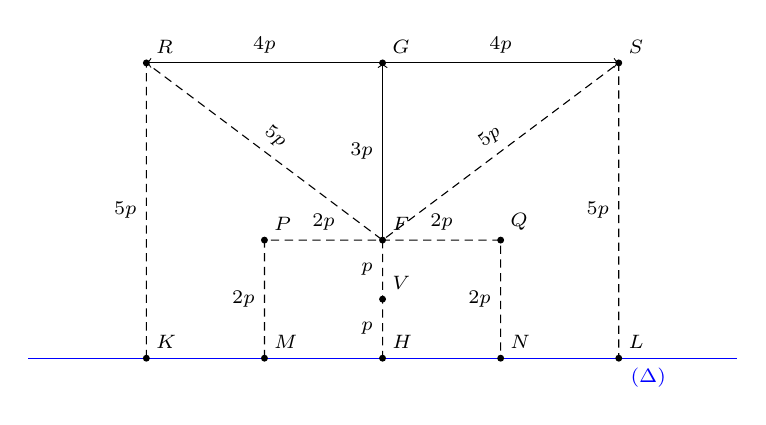
\begin{tikzpicture}[x=.75cm,y=.75cm,every node/.append style={font=\scriptsize}]
    \coordinate(D')at(-6,-1);
    \coordinate(D)at(6,-1);
    \coordinate(F)at(0,1);
    \coordinate(H)at(0,-1);
    \coordinate(V)at(0,0);
    \coordinate(M)at(-2,-1);
    \coordinate(P)at(-2,1);
    \coordinate(Q)at(2,1);
    \coordinate(N)at(2,-1);
    \coordinate(G)at(0,4);
    \coordinate(R)at(-4,4);
    \coordinate(S)at(4,4);
    \coordinate(K)at(-4,-1);
    \coordinate(L)at(4,-1);
    \tkzMarkRightAngles(F,H,D' P,M,D' Q,N,D' F,G,R R,K,D' S,L,D')
    \draw[color=blue](D')--node[sloped,very near end,below]{$ (\Delta) $}(D);
    \draw[densely dashed]
    (F)--node[left]{$ p $}(V)--node[left]{$ p $}(H)
    (M)--node[left]{$ 2p $}(P)--node[above]{$ 2p $}(F)--node[above]{$ 2p $}(Q)--node[left]{$ 2p $}(N)
    (K)--node[left]{$ 5p $}(R)--node[sloped,above]{$ 5p $}(F)--node[sloped,above]{$ 5p $}(S)--node[left]{$ 5p $}(L);
    \foreach\p in {F,H,V,M,N,P,Q,G,R,S,K,L}{%
      \fill[color=black](\p)circle(1.25pt)node[above right]{$ \p $};}
    \tkzMarkSegments[mark=s|,size=3pt](F,V V,H)
    \tkzMarkSegments[mark=s||,size=3pt](M,P P,F F,Q Q,N)
    \tkzMarkSegments[mark=o,size=2pt](K,R R,F F,S S,L)
    \draw[->](F)--node[left]{$ 3p $}(G);
    \foreach\p in {R,S}{%
      \draw[->](G)--node[above]{$ 4p $}(\p);}
    \end{tikzpicture}
  \end{figure}
  \item គូសខ្សែកោងកាត់តាមចំណុច $ R,P,V,Q $ និង $ S $ ដូចខាងក្រោម
  \begin{figure}[H]
    \centering
    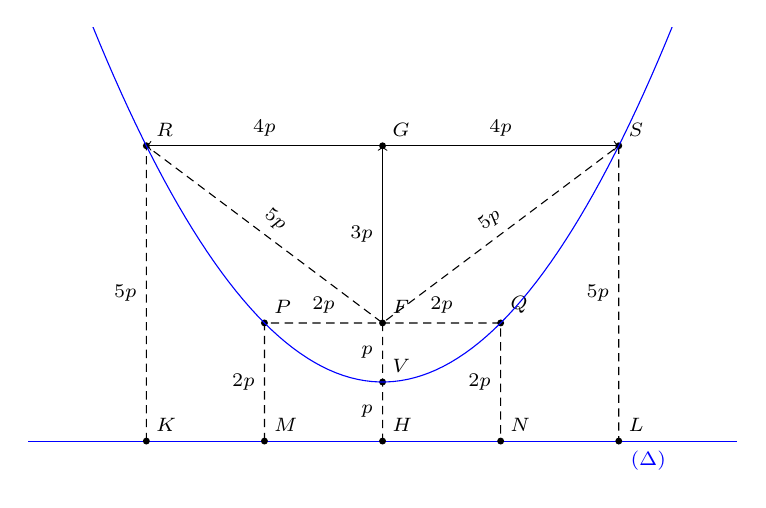
\begin{tikzpicture}[x=.75cm,y=.75cm,every node/.append style={font=\scriptsize}]
    \coordinate(D')at(-6,-1);
    \coordinate(D)at(6,-1);
    \coordinate(F)at(0,1);
    \coordinate(H)at(0,-1);
    \coordinate(V)at(0,0);
    \coordinate(M)at(-2,-1);
    \coordinate(P)at(-2,1);
    \coordinate(Q)at(2,1);
    \coordinate(N)at(2,-1);
    \coordinate(G)at(0,4);
    \coordinate(R)at(-4,4);
    \coordinate(S)at(4,4);
    \coordinate(K)at(-4,-1);
    \coordinate(L)at(4,-1);
    \tkzMarkRightAngles(F,H,D' P,M,D' Q,N,D' F,G,R R,K,D' S,L,D')
    \draw[color=blue](D')--node[sloped,very near end,below]{$ (\Delta) $}(D);
    \draw[densely dashed]
    (F)--node[left]{$ p $}(V)--node[left]{$ p $}(H)
    (M)--node[left]{$ 2p $}(P)--node[above]{$ 2p $}(F)--node[above]{$ 2p $}(Q)--node[left]{$ 2p $}(N)
    (K)--node[left]{$ 5p $}(R)--node[sloped,above]{$ 5p $}(F)--node[sloped,above]{$ 5p $}(S)--node[left]{$ 5p $}(L);
    \foreach\p in {F,H,V,M,N,P,Q,G,R,S,K,L}{%
      \fill[color=black](\p)circle(1.25pt)node[above right]{$ \p $};}
    \tkzMarkSegments[mark=s|,size=3pt](F,V V,H)
    \tkzMarkSegments[mark=s||,size=3pt](M,P P,F F,Q Q,N)
    \tkzMarkSegments[mark=o,size=2pt](K,R R,F F,S S,L)
    \draw[->](F)--node[left]{$ 3p $}(G);
    \foreach\p in {R,S}{%
      \draw[->](G)--node[above]{$ 4p $}(\p);}
    \clip(-6,-1) rectangle (6,6);
    \draw[color=blue,domain=-6:6,samples=100] plot(\x,{.25*\x*\x});
    \end{tikzpicture}
  \end{figure}
  ខ្សែកោងដែលសង់បានជាប៉ារ៉ាបូលដែលមានកំណុំ $ F $ និងបន្ទាត់ប្រាប់ទិស $ (\Delta) $
\end{enumerate}
\section{សមីការស្តង់ដានៃប៉ារ៉ាបូល}
\subsection{បន្ទាត់ប្រាប់ទិសស្របអ័ក្សអាប់ស៊ីស}
\begin{generality}
	ប៉ារ៉ាបូល $ (P) $ ដែលមានកំពូលត្រង់ចំណុច $ V(h,k) $ និងបន្ទាត់ប្រាប់ទិស $ (\Delta): y=k-p $ មានសមីការស្តង់ដា
	\begin{equation}
	(P):(x-h)^2=4p(y-k)
	\end{equation}
	ហើយមានកំណុំ $ F(h,k+p) $~។
\end{generality}
%
\begin{figure}[H]
	\caption{ប៉ារ៉ាបូល $ (x-h)^2=4p(y-k) $}
	\begin{subfigure}[t]{.5\textwidth}
		\centering
		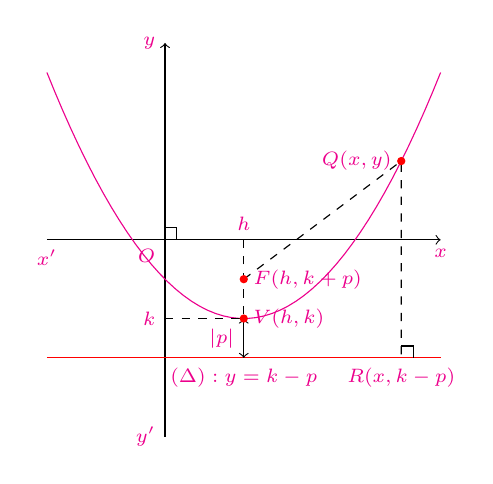
\begin{tikzpicture}[every node/.style={font=\scriptsize,text=magenta}]
		\coordinate(O)at(0,0);
		\coordinate(X')at(-1.5,0);
		\coordinate(X)at(3.5,0);
		\coordinate(Y')at(0,-2.5);
		\coordinate(Y)at(0,2.5);
		\coordinate(V)at(1,-1);
		\coordinate(F)at(1,-.5);
		\coordinate(D)at(1,-1.5);
		\coordinate(Q)at(3,1);
		\draw[->](X')node[below]{$ x' $}--(X)node[below]{$ x $};
		\draw[->](Y')node[left]{$ y' $}--(Y)node[left]{$ y $};
		\draw([yshift=1ex]O)--([xshift=1ex,yshift=1ex]O)--([xshift=1ex]O);
		\draw[magenta] plot[samples=50,domain=-1.5:3.5](\x,{\x*(.5*\x-1)-.5});
		\draw[red](D-|X')--node[midway,below]{$ (\Delta):y=k-p $}(D-|X);
		\draw[dashed](V-|Y)--(V)--(V|-X);
		\draw[dashed](F)--(Q)--(Q|-D);
		\draw([yshift=1ex]Q|-D)--([xshift=1ex,yshift=1ex]Q|-D)--([xshift=1ex]Q|-D);
		\draw[<->](V)--node[left]{$ |p| $}(V|-D);
		\node[below left]at(O){$ O $};
		\node[right]at(V){$ V(h,k) $};
		\node[right]at(F){$ F(h,k+p) $};
		\node[above]at(V|-X){$ h $};
		\node[left]at(V-|Y){$ k $};
		\node[left]at(Q){$ Q(x,y) $};
		\node[below]at(Q|-D){$ R(x,k-p) $};
%		\node[right]at(0,1.5){$ (x-h)^2=4p(y-k) $};
		\foreach\p in{V,F,Q}\fill[red](\p)circle(1.5pt);
    \coordinate(R)at(Q|-D);
    \tkzMarkSegments[mark=||,color=blue](F,Q Q,R)
		\end{tikzpicture}
		\subcaption{ករណី $ p>0 $}
	\end{subfigure}
	%
	\begin{subfigure}[t]{.5\textwidth}
		\centering
		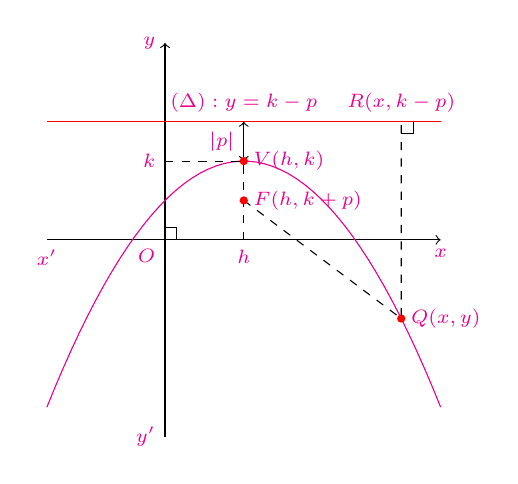
\begin{tikzpicture}[every node/.style={font=\scriptsize,text=magenta}]
		\coordinate(O)at(0,0);
		\coordinate(X')at(-1.5,0);
		\coordinate(X)at(3.5,0);
		\coordinate(Y')at(0,-2.5);
		\coordinate(Y)at(0,2.5);
		\coordinate(V)at(1,1);
		\coordinate(F)at(1,.5);
		\coordinate(D)at(1,1.5);
		\coordinate(Q)at(3,-1);
		\draw[->](X')node[below]{$ x' $}--(X)node[below]{$ x $};
		\draw[->](Y')node[left]{$ y' $}--(Y)node[left]{$ y $};
		\draw([yshift=1ex]O)--([xshift=1ex,yshift=1ex]O)--([xshift=1ex]O);
		\draw[magenta] plot[samples=50,domain=-1.5:3.5](\x,{\x*(-.5*\x+1)+.5});
		\draw[red](D-|X')--node[midway,above]{$ (\Delta):y=k-p $}(D-|X);
		\draw[dashed](V-|Y)--(V)--(V|-X);
		\draw[dashed](F)--(Q)--(Q|-D);
		\draw([yshift=-1ex]Q|-D)--([xshift=1ex,yshift=-1ex]Q|-D)--([xshift=1ex]Q|-D);
		\draw[<->](V)--node[left]{$ |p| $}(V|-D);
		\node[below left]at(O){$ O $};
		\node[right]at(V){$ V(h,k) $};
		\node[right]at(F){$ F(h,k+p) $};
		\node[below]at(V|-X){$ h $};
		\node[left]at(V-|Y){$ k $};
		\node[right]at(Q){$ Q(x,y) $};
		\node[above]at(Q|-D){$ R(x,k-p) $};
%		\node[right]at(0,-1.5){$ (x-h)^2=4p(y-k) $};
		\foreach\p in{V,F,Q}\fill[red](\p)circle(1.5pt);
    \coordinate(R)at(Q|-D);
    \tkzMarkSegments[mark=||,color=blue](F,Q Q,R)
		\end{tikzpicture}
		\subcaption{ករណី $ p<0 $}
	\end{subfigure}
\end{figure}
%
\begin{proof}
	តាង $ Q(x,y) $ ជាចំណុចនៅលើប៉ារ៉ាបូលដែលមានកំណុំ $ F(h,k+p) $ និងបន្ទាត់ប្រាប់ទិស $ (\Delta):y=k-p $ និង $ R(x,k-p) $ ជាចំណោលកែងនៃចំណុច $ Q $ លើបន្ទាត់ $ (\Delta) $ នោះយើងបាន
	\begin{align*}
		FQ &= QR\\
		\sqrt{(x-h)^2+(y-k-p)^2} &= \sqrt{(x-x)^2+(y-k+p)^2}\\
		(x-h)^2+(y-k-p)^2 &= (y-k+p)^2\\
		(x-h)^2 &= (y-k+p)^2-(y-k-p)^2\\
		(x-h)^2 &= (2p)(2y-2k)\\
		\therefore (x-h)^2 &= 4p(y-k)
	\end{align*}
\end{proof}
%
\begin{example}
	សរសេរសមីការស្តង់ដានៃប៉ារ៉ាបូល $ (P) $ ដែលមានកំពូល\\ $ V(3,2) $ និងបន្ទាត់ប្រាប់ទិស $ (\Delta):y=1 $~។
\end{example}
%
\begin{proof}
	ប៉ារ៉ាបូល $ (P) $ មានបន្ទាត់ប្រាប់ទិស $ (\Delta):y=1 $ ស្របនឹងអ័ក្សអាប់ស៊ីស​ នោះវាមានសមីការស្តង់ដា $ (P):(x-h)^2=4p(y-k) $~។
	\begin{itemize}
		\item កំពូល $ V(3,2) $ នោះ $ h=3 $ និង $ k=2 $
		\item បន្ទាត់ប្រាប់ទិស $ y=1 $ នោះ $ k-p=1 $ នាំឲ្យ $ p=k-1=2-1=1 $
	\end{itemize}
	ដូច្នេះ ប៉ារ៉ាបូលមានសមីការស្តង់ដា $ (P):(x-3)^2=4(1)(y-2) $~។
\end{proof}
%
\begin{example}
	សរសេរសមីការស្តង់ដានៃប៉ារ៉ាបូលដែលមានកំពូល $ (-1,1) $ និងបន្ទាត់ប្រាប់ទិស $ y=2 $~។
\end{example}
%
\begin{proof}
	ប៉ារ៉ាបូលមានបន្ទាត់ប្រាប់ទិស $ y=2 $ ស្របនឹងអ័ក្សអាប់ស៊ីស​ នោះវាមានសមីការស្តង់ដា $ (x-h)^2=4p(y-k) $~។
	\begin{itemize}
		\item កំពូល $ (-1,1) $ នោះ $ h=-1 $ និង $ k=1 $
		\item បន្ទាត់ប្រាប់ទិស $ y=2 $ នោះ $ k-p=2 $ នាំឲ្យ $ p=k-2=1-2=-1 $
	\end{itemize}
	ដូច្នេះ ប៉ារ៉ាបូលមានសមីការស្តង់ដា $ (x+1)^2=4(-1)(y-1) $~។
\end{proof}
%
\begin{example}
	សរសេរសមីការស្តង់ដានៃប៉ារ៉ាបូលដែលមានកំពូល $ (-2,-1) $ និងបន្ទាត់ប្រាប់ទិស $ y=-2 $~។
\end{example}
%
\begin{proof}
	ប៉ារ៉ាបូលមានបន្ទាត់ប្រាប់ទិស $ y=-2 $ ស្របនឹងអ័ក្សអាប់ស៊ីស​ នោះវាមានសមីការស្តង់ដា $ (x-h)^2=4p(y-k) $~។
	\begin{itemize}
		\item កំពូល $ (-2,-1) $ នោះ $ h=-2 $ និង $ k=-1 $
		\item បន្ទាត់ប្រាប់ទិស $ y=-2 $ នោះ $ k-p=-2 $ នាំឲ្យ $ p=k+2=-1+2=1 $
	\end{itemize}
	ដូច្នេះ ប៉ារ៉ាបូលមានសមីការស្តង់ដា $ (x+2)^2=4(1)(y+1) $~។
\end{proof}
%
\subsection{បន្ទាត់ប្រាប់ទិសស្របអ័ក្សអរដោនេ}
%
\begin{generality}
	ប៉ារ៉ាបូល $ (P) $ ដែលមានកំពូលត្រង់ចំណុច $ V(h,k) $ និងបន្ទាត់ប្រាប់ទិស $ (\Delta): x=h-p $ មានសមីការស្តង់ដា
	\begin{equation}
		 (P):(y-k)^2=4p(x-h)
	\end{equation}
	ហើយមានកំណុំ $ F(h+p,k) $~។
\end{generality}
%
\begin{figure}[H]
	\caption{ប៉ារ៉ាបូល $ (y-k)^2=4p(x-h) $}
	\begin{subfigure}[b]{.5\textwidth}
		\centering
		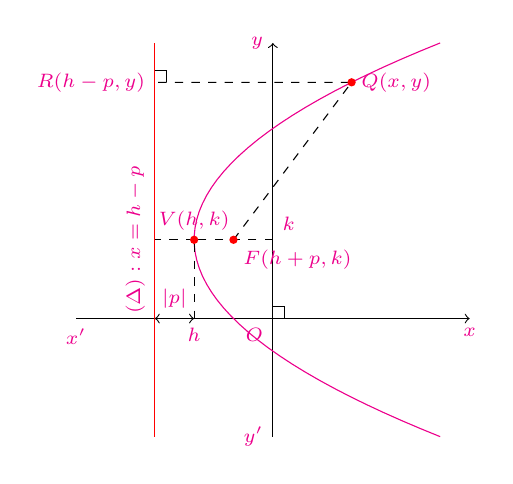
\begin{tikzpicture}[every node/.style={font=\scriptsize,text=magenta}]
		\coordinate(O)at(0,0);
		\coordinate(X')at(-2.5,0);
		\coordinate(X)at(2.5,0);
		\coordinate(Y')at(0,-1.5);
		\coordinate(Y)at(0,3.5);
		\coordinate(V)at(-1,1);
		\coordinate(F)at(-.5,1);
		\coordinate(D)at(-1.5,1);
		\coordinate(Q)at(1,3);
		\draw[->](X')node[below]{$ x' $}--(X)node[below]{$ x $};
		\draw[->](Y')node[left]{$ y' $}--(Y)node[left]{$ y $};
		\draw([yshift=1ex]O)--([xshift=1ex,yshift=1ex]O)--([xshift=1ex]O);
		\draw[magenta] plot[samples=50,domain=-1.5:3.5]({\x*(.5*\x-1)-.5},\x);
		\draw[red](D|-Y')--node[sloped,midway,above]{$ (\Delta):x=h-p $}(D|-Y);
		\draw[dashed](V-|Y)--(V)--(V|-X);
		\draw[dashed](F)--(Q)--(Q-|D);
		\draw([xshift=1ex]Q-|D)--([xshift=1ex,yshift=1ex]Q-|D)--([yshift=1ex]Q-|D);
		\draw[dashed](V)--(V-|D);
		\node[below left]at(O){$ O $};
		\node[above]at(V){$ V(h,k) $};
		\node[below right]at(F){$ F(h+p,k) $};
		\node[below]at(V|-X){$ h $};
		\node[above right]at(V-|Y){$ k $};
		\node[right]at(Q){$ Q(x,y) $};
		\node[left]at(Q-|D){$ R(h-p,y) $};
		%		\node[left] at(0,1.5){$ (y-k)^2=4p(x-h) $};
		\draw[<->](V|-X)--node[above]{$ |p| $}(D|-X);
		\foreach\p in{V,F,Q}\fill[red](\p)circle(1.5pt);
    \coordinate(R)at(Q-|D);
    \tkzMarkSegments[mark=||,color=blue](F,Q Q,R)
		\end{tikzpicture}
		\subcaption{ករណី $ p>0 $}
	\end{subfigure}
	%
	\begin{subfigure}[b]{.5\textwidth}
		\centering
		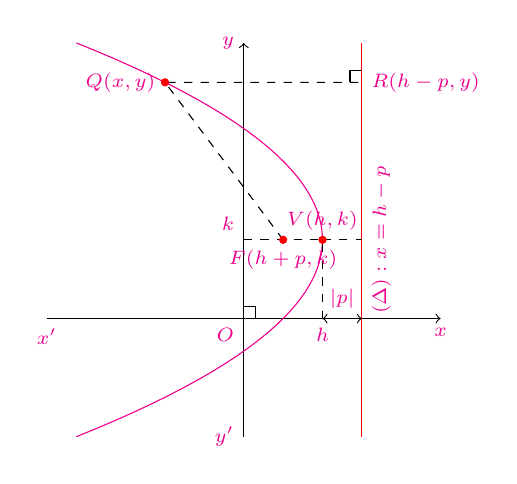
\begin{tikzpicture}[every node/.style={font=\scriptsize,text=magenta}]
		\coordinate(O)at(0,0);
		\coordinate(X')at(-2.5,0);
		\coordinate(X)at(2.5,0);
		\coordinate(Y')at(0,-1.5);
		\coordinate(Y)at(0,3.5);
		\coordinate(V)at(1,1);
		\coordinate(F)at(.5,1);
		\coordinate(D)at(1.5,1);
		\coordinate(Q)at(-1,3);
		\draw[->](X')node[below]{$ x' $}--(X)node[below]{$ x $};
		\draw[->](Y')node[left]{$ y' $}--(Y)node[left]{$ y $};
		\draw([yshift=1ex]O)--([xshift=1ex,yshift=1ex]O)--([xshift=1ex]O);
		\draw[magenta] plot[samples=50,domain=-1.5:3.5]({\x*(-.5*\x+1)+.5},\x);
		\draw[red](D|-Y')--node[sloped,midway,below]{$ (\Delta):x=h-p $}(D|-Y);
		\draw[dashed](V-|Y)--(V)--(V|-X);
		\draw[dashed](F)--(Q)--(Q-|D);
		\draw([xshift=-1ex]Q-|D)--([xshift=-1ex,yshift=1ex]Q-|D)--([yshift=1ex]Q-|D);
		\draw[dashed](V)--(V-|D);
		\node[below left]at(O){$ O $};
		\node[above]at(V){$ V(h,k) $};
		\node[below]at(F){$ F(h+p,k) $};
		\node[below]at(V|-X){$ h $};
		\node[above left]at(V-|Y){$ k $};
		\node[left]at(Q){$ Q(x,y) $};
		\node[right]at(Q-|D){$ R(h-p,y) $};
%		\node[left] at(0,1.5){$ (y-k)^2=4p(x-h) $};
		\draw[<->](V|-X)--node[above]{$ |p| $}(D|-X);
		\foreach\p in{V,F,Q}\fill[red](\p)circle(1.5pt);
    \coordinate(R)at(Q-|D);
    \tkzMarkSegments[mark=||,color=blue](F,Q Q,R)
		\end{tikzpicture}
		\subcaption{ករណី $ p<0 $}
	\end{subfigure}
\end{figure}
%
\begin{proof}
	តាង $ Q(x,y) $ ជាចំណុចនៅលើប៉ារ៉ាបូលដែលមានកំណុំ $ F(h+p,k) $ និងបន្ទាត់ប្រាប់ទិស $ (\Delta):x=h-p $ និង $ R(h-p,y) $ ជាចំណោលកែងនៃចំណុច $ Q $ លើបន្ទាត់ $ (\Delta) $ នោះយើងបាន
	\begin{align*}
	FQ &= QR\\
	\sqrt{(x-h-p)^2+(y-k)^2} &= \sqrt{(x-h+p)^2+(y-y)^2}\\
	(x-h-p)^2+(y-k)^2 &= (x-h+p)^2\\
	(y-k)^2 &= (x-h+p)^2-(x-h-p)^2\\
	(y-k)^2 &= (2p)(2x-2h)\\
	\therefore (y-k)^2 &= 4p(x-h)
	\end{align*}
\end{proof}
%
\begin{example}
	សរសេរសមីការស្តង់ដានៃប៉ារ៉ាបូល $ (P) $ ដែលមានកំពូល\\ $ V(-1,2) $ និងបន្ទាត់ប្រាប់ទិស $ (\Delta):x=1 $~។
\end{example}
%
\begin{proof}
	ប៉ារ៉ាបូល $ (P) $ មានបន្ទាត់ប្រាប់ទិស $ (\Delta):x=1 $ ស្របនឹងអ័ក្សអរដោនេ នោះវាមានសមីការស្តង់ដា $ (P):(y-k)^2=4p(x-h) $~។
	\begin{itemize}
		\item កំពូល $ V(-1,2) $ នោះ $ h=-1 $ និង $ k=2 $
		\item បន្ទាត់ប្រាប់ទិស $ x=1 $ នោះ $ h-p=1 $ នាំឲ្យ $ p=h-1=-1-1=-2 $
	\end{itemize}
	ដូច្នេះ ប៉ារ៉ាបូលមានសមីការស្តង់ដា $ (P):(y-2)^2=4(-2)(x+1) $~។
\end{proof}
%
\begin{example}
	សរសេរសមីការស្តង់ដានៃប៉ារ៉ាបូលដែលមានកំពូល $ (-2,-1) $ និងបន្ទាត់ប្រាប់ទិស $ x=0 $~។
\end{example}
%
\begin{proof}
	ប៉ារ៉ាបូលមានបន្ទាត់ប្រាប់ទិស $ x=0 $ ស្របនឹងអ័ក្សអរដោនេ នោះវាមានសមីការស្តង់ដា $ (y-k)^2=4p(x-h) $~។
	\begin{itemize}
		\item កំពូល $ (-2,-1) $ នោះ $ h=-2 $ និង $ k=-1 $
		\item បន្ទាត់ប្រាប់ទិស $ x=0 $ នោះ $ h-p=0 $ នាំឲ្យ $ p=h=-2 $
	\end{itemize}
	ដូច្នេះ ប៉ារ៉ាបូលមានសមីការស្តង់ដា $ (y+1)^2=4(-2)(x+2) $~។
\end{proof}
%
\begin{example}
	សរសេរសមីការស្តង់ដានៃប៉ារ៉ាបូលដែលមានកំពូល $ (4,2) $ និងបន្ទាត់ប្រាប់ទិស $ x=3 $~។
\end{example}
%
\begin{proof}
	ប៉ារ៉ាបូលមានបន្ទាត់ប្រាប់ទិស $ x=3 $ ស្របនឹងអ័ក្សអរដោនេ នោះវាមានសមីការស្តង់ដា $ (y-k)^2=4p(x-h) $~។
	\begin{itemize}
		\item កំពូល $ (4,2) $ នោះ $ h=4 $ និង $ k=2 $
		\item បន្ទាត់ប្រាប់ទិស $ x=3 $ នោះ $ h-p=3 $ នាំឲ្យ $ p=h-3=4-3=1 $
	\end{itemize}
	ដូច្នេះ ប៉ារ៉ាបូលមានសមីការស្តង់ដា $ (y-2)^2=4(1)(x-4) $~។
\end{proof}
%
%\newpage
\begin{generality}
	ប៉ារ៉ាបូល $ (P) $ ដែលមានសមីការស្តង់ដា
	\begin{itemize}
		\item  $ (P):(x-h)^2=4p(y-k) $ មាន $ \begin{dcases}
			\text{កំពូល}\; V(h,k)\\
			\text{កំណុំ}\; F(h,k+p)\\
			\text{បន្ទាត់ប្រាប់ទិស}\; (\Delta):y=k-p
		\end{dcases} $
		\item  $ (P):(y-k)^2=4p(x-h) $ មាន $ \begin{dcases}
			\text{កំពូល}\; V(h,k)\\
			\text{កំណុំ}\; F(h+p,k)\\
			\text{បន្ទាត់ប្រាប់ទិស}\; (\Delta):x=h-p
		\end{dcases} $
	\end{itemize}
\end{generality}
%
\section{សមីការទូទៅនៃប៉ារ៉ាបូល}
\subsection{បន្ទាត់ប្រាប់ទិសស្របអ័ក្សអាប់ស៊ីស}
ពន្លាតសមីការស្ដង់ដា $ (P):(x-h)^2=4p(y-k) $ នៃប៉ារ៉ាបូលដែលមានកំពូល $ V(h,k) $ កំណុំ $ F(h,k+p) $ និងបន្ទាត់ប្រាប់ទិស $ (\Delta):y=k-p $ យើងបាន
\begin{align*}
	(x-h)^2 &=4p(y-k)\\
	x^2-2hx+h^2 &= 4py-4pk\\
	x^2-2hx-4py+(h^2+4pk) &=0
\end{align*}
%
\begin{generality}
	ប៉ារ៉ាបូលដែលមានបន្ទាត់ប្រាប់ទិសស្របនឹងអ័ក្សអាប់ស៊ីសមានសមីការទូទៅ
	\begin{equation}
		Ax^2+Cx+Dy+E=0
	\end{equation}
	ដែល $ A,C,D,E $ ជាចំនួនពិត និង $ A\neq 0 $~។
\end{generality}
%
\begin{example}
	ចូរកណត់ កូអរដោនេ​កំពូល កូអរដោនេ​កំណុំ និង សរសេរសមីការប្រាប់ទិស នៃប៉ារ៉ាបូលដែលមានសមីការ $ y=x^2+2x+2 $~។
\end{example}
%
\begin{proof}
	សមីការ $ y=x^2+2x+2 $ មានដឺក្រេទី២ ជាដឺក្រេនៃអថេរ $ x $ នោះវាជាសមីការទូទៅនៃប៉ារ៉ាបូលដែលមានបន្ទាត់ប្រាប់ទិសស្របនឹងអ័ក្សអាប់ស៊ីស នាំឲ្យសមីការស្តង់ដារបស់វាមានទម្រង់ $ (x-h)^2=4p(y-k) $ និង
	\begin{itemize}
		\item កំពូល $ (h,k) $
		\item កំណុំ $ (h,k+p) $
		\item បន្ទាត់ប្រាប់ទិស $ y=k-p $
	\end{itemize}
	ដោយសមីការទូទៅអាចសរសេរជា
	\begin{align*}
		x^2+2x+2 &=y\\
		x^2+2x+1 &=y-1\\
		(x+1)^2 &=4\left(\dfrac{1}{4}\right)(y-1)
	\end{align*}
	ផ្ទឹមនឹងសមីការស្តង់ដា $ (x-h)^2=4p(y-k) $ យើងបាន $ h=-1,k=1 $ និង $ p=\dfrac{1}{4} $~។ ដូច្នេះ ប៉ារ៉ាបូលមាន​ កំពូល $ (-1,1) $ កំណុំ $ \left(-1,\dfrac{5}{4}\right) $ និង បន្ទាត់ប្រាប់ទិស $ y=\dfrac{3}{4} $~។
\end{proof}
%
\begin{example}
	ចូរកណត់ កូអរដោនេ​កំពូល កូអរដោនេ​កំណុំ និង សរសេរសមីការប្រាប់ទិស នៃប៉ារ៉ាបូលដែលមានសមីការ $ y=-x^2-4x $~។
\end{example}
%
\begin{proof}
	សមីការ $ y=-x^2-4x $ មានដឺក្រេទី២ ជាដឺក្រេនៃអថេរ $ x $ នោះវាជាសមីការទូទៅនៃប៉ារ៉ាបូលដែលមានបន្ទាត់ប្រាប់ទិសស្របនឹងអ័ក្សអាប់ស៊ីស នាំឲ្យសមីការស្តង់ដារបស់វាមានទម្រង់ $ (x-h)^2=4p(y-k) $ និង
	\begin{itemize}
		\item កំពូល $ (h,k) $
		\item កំណុំ $ (h,k+p) $
		\item បន្ទាត់ប្រាប់ទិស $ y=k-p $
	\end{itemize}
	ដោយសមីការទូទៅអាចសរសេរជា
	\begin{align*}
	x^2+4x &=-y\\
	x^2+4x+4 &=-y+4\\
	(x+2)^2 &=4\left(-\dfrac{1}{4}\right)(y-4)
	\end{align*}
	ផ្ទឹមនឹងសមីការស្តង់ដា $ (x-h)^2=4p(y-k) $ យើងបាន $ h=-2,k=4 $ និង $ p=-\dfrac{1}{4} $~។ ដូច្នេះ ប៉ារ៉ាបូលមាន​ កំពូល $ (-2,4) $ កំណុំ $ \left(-2,\dfrac{15}{4}\right) $ និង បន្ទាត់ប្រាប់ទិស $ y=\dfrac{17}{4} $~។
\end{proof}
%
\begin{example}
	ចូរកណត់ កូអរដោនេ​កំពូល កូអរដោនេ​កំណុំ និង សរសេរសមីការប្រាប់ទិស នៃប៉ារ៉ាបូលដែលមានសមីការ $ x^2-6x+4y+5=0 $~។
\end{example}
%
\begin{proof}
	សមីការ $ x^2-6x+4y+5=0 $ មានដឺក្រេទី២ ជាដឺក្រេនៃអថេរ $ x $ នោះវាជាសមីការទូទៅនៃប៉ារ៉ាបូលដែលមានបន្ទាត់ប្រាប់ទិសស្របនឹងអ័ក្សអាប់ស៊ីស នាំឲ្យសមីការស្តង់ដារបស់វាមានទម្រង់ $ (x-h)^2=4p(y-k) $ និង
	\begin{itemize}
		\item កំពូល $ (h,k) $
		\item កំណុំ $ (h,k+p) $
		\item បន្ទាត់ប្រាប់ទិស $ y=k-p $
	\end{itemize}
	ដោយសមីការទូទៅអាចសរសេរជា
	\begin{align*}
	x^2-6x+4y+5 &=0\\
	x^2-6x+9 &=-4y+4\\
	(x-3)^2 &=4(-1)(y-1)
	\end{align*}
	ផ្ទឹមនឹងសមីការស្តង់ដា $ (x-h)^2=4p(y-k) $ យើងបាន $ h=3,k=1 $ និង $ p=-1 $~។ ដូច្នេះ ប៉ារ៉ាបូលមាន​ កំពូល $ (3,1) $ កំណុំ $ (3,0) $ និង បន្ទាត់ប្រាប់ទិស $ y=2 $~។
\end{proof}
%
\subsection{បន្ទាត់ប្រាប់ទិសស្របអ័ក្សអរដោនេ}
ពន្លាតសមីការស្ដង់ដា $ (P):(y-k)^2=4p(x-h) $ នៃប៉ារ៉ាបូលដែលមានកំពូល $ V(h,k) $ កំណុំ $ F(h+p,k) $ និងបន្ទាត់ប្រាប់ទិស $ (\Delta):x=h-p $ យើងបាន
\begin{align*}
(y-k)^2 &=4p(x-h)\\
y^2-2ky+k^2 &= 4px-4ph\\
y^2-2ky-4px+(k^2+4ph) &=0
\end{align*}
%
\begin{generality}
	ប៉ារ៉ាបូលដែលមានបន្ទាត់ប្រាប់ទិសស្របនឹងអ័ក្សអរដោនេមានសមីការទូទៅ
	\begin{equation}
	By^2+Cx+Dy+E=0
	\end{equation}
	ដែល $ B,C,D,E $ ជាចំនួនពិត និង $ B\neq 0 $~។
\end{generality}
%
\begin{example}
	ចូរកណត់ កូអរដោនេ​កំពូល កូអរដោនេ​កំណុំ និង សរសេរសមីការប្រាប់ទិស នៃប៉ារ៉ាបូលដែលមានសមីការ $ y^2+4x+8y+8=0 $~។
\end{example}
%
\begin{proof}
	សមីការ $ y^2+4x+8y+8=0 $ មានដឺក្រេទី២ ជាដឺក្រេនៃអថេរ $ y $ នោះវាជាសមីការទូទៅនៃប៉ារ៉ាបូលដែលមានបន្ទាត់ប្រាប់ទិសស្របនឹងអ័ក្សអរដោនេ នាំឲ្យសមីការស្តង់ដារបស់វាមានទម្រង់ $ (y-k)^2=4p(x-h) $ និង
	\begin{itemize}
		\item កំពូល $ (h,k) $
		\item កំណុំ $ (h+p,k) $
		\item បន្ទាត់ប្រាប់ទិស $ x=h-p $
	\end{itemize}
	ដោយសមីការទូទៅអាចសរសេរជា
	\begin{align*}
	y^2+4x+8y+8 &=0\\
	y^2+8y+16 &=-4x+8\\
	(y+4)^2 &=4(-1)(x-2)
	\end{align*}
	ផ្ទឹមនឹងសមីការស្តង់ដា $ (y-k)^2=4p(x-h) $ យើងបាន $ h=2,k=-4 $ និង $ p=-1 $~។ ដូច្នេះ ប៉ារ៉ាបូលមាន​ កំពូល $ (2,-4) $ កំណុំ $ (1,-4) $ និង បន្ទាត់ប្រាប់ទិស $ x=3 $~។
\end{proof}
%
\begin{example}
	ចូរកណត់ កូអរដោនេ​កំពូល កូអរដោនេ​កំណុំ និង សរសេរសមីការប្រាប់ទិស នៃប៉ារ៉ាបូលដែលមានសមីការ $ y^2-8x-10y+1=0 $~។
\end{example}
%
\begin{proof}
	សមីការ $ y^2-8x-10y+1=0 $ មានដឺក្រេទី២ ជាដឺក្រេនៃអថេរ $ y $ នោះវាជាសមីការទូទៅនៃប៉ារ៉ាបូលដែលមានបន្ទាត់ប្រាប់ទិសស្របនឹងអ័ក្សអរដោនេ នាំឲ្យសមីការស្តង់ដារបស់វាមានទម្រង់ $ (y-k)^2=4p(x-h) $ និង
	\begin{itemize}
		\item កំពូល $ (h,k) $
		\item កំណុំ $ (h+p,k) $
		\item បន្ទាត់ប្រាប់ទិស $ x=h-p $
	\end{itemize}
	ដោយសមីការទូទៅអាចសរសេរជា
	\begin{align*}
	y^2-8x-10y+1 &=0\\
	y^2-10y+25 &=8x+24\\
	(y-5)^2 &=4(2)(x+3)
	\end{align*}
	ផ្ទឹមនឹងសមីការស្តង់ដា $ (y-k)^2=4p(x-h) $ យើងបាន $ h=-3,k=5 $ និង $ p=2 $~។ ដូច្នេះ ប៉ារ៉ាបូលមាន​ កំពូល $ (-3,5) $ កំណុំ $ (-1,5) $ និង បន្ទាត់ប្រាប់ទិស $ x=-5 $~។
\end{proof}
%
\begin{example}
	ចូរកណត់ កូអរដោនេ​កំពូល កូអរដោនេ​កំណុំ និង សរសេរសមីការប្រាប់ទិស នៃប៉ារ៉ាបូលដែលមានសមីការ $ y^2+x+y+1=0 $~។
\end{example}
%
\begin{proof}
	សមីការ $ y^2+x+y+1=0 $ មានដឺក្រេទី២ ជាដឺក្រេនៃអថេរ $ y $ នោះវាជាសមីការទូទៅនៃប៉ារ៉ាបូលដែលមានបន្ទាត់ប្រាប់ទិសស្របនឹងអ័ក្សអរដោនេ នាំឲ្យសមីការស្តង់ដារបស់វាមានទម្រង់ $ (y-k)^2=4p(x-h) $ និង
	\begin{itemize}
		\item កំពូល $ (h,k) $
		\item កំណុំ $ (h+p,k) $
		\item បន្ទាត់ប្រាប់ទិស $ x=h-p $
	\end{itemize}
	ដោយសមីការទូទៅអាចសរសេរជា
	\begin{align*}
	y^2+x+y+1 &=0\\
	y^2+y &=-x-1\\
	y^2+2y\left(\dfrac{1}{2}\right)+\left(\dfrac{1}{2}\right)^2 &=-x-1+\left(\dfrac{1}{2}\right)^2\\
	\left(y+\dfrac{1}{2}\right)^2 &=-\left(x+\dfrac{3}{4}\right)\\
	\left(y+\dfrac{1}{2}\right)^2 &=4\left(-\dfrac{1}{4}\right)\left(x+\dfrac{3}{4}\right)
	\end{align*}
	ផ្ទឹមនឹងសមីការស្តង់ដា $ (y-k)^2=4p(x-h) $ យើងបាន $ h=-\dfrac{3}{4},k=-\dfrac{1}{2} $ និង $ p=-\dfrac{1}{4} $~។ ដូច្នេះ ប៉ារ៉ាបូលមាន​ កំពូល $ \left(-\dfrac{3}{4},-\dfrac{1}{2}\right) $ កំណុំ $ \left(-1,-\dfrac{1}{2}\right) $ និង បន្ទាត់ប្រាប់ទិស $ x=-\dfrac{1}{2} $~។
\end{proof}
%
\section{អ័ក្សឆ្លុះនៃប៉ារ៉ាបូល}
\begin{generality}
	បន្ទាត់ដែលកាត់តាម កំពូល និង កំណុំ នៃប៉ារ៉ាបូលជា \emph{អ័ក្សឆ្លុះ}។ អ័ក្សឆ្លុះនៃប៉ារ៉ាបូលមួយ កែងនឹងបន្ទាត់ប្រាប់ទិសនៃប៉ារ៉ាបូលនោះ។
\end{generality}
%
\begin{example}
	សរសេរសមីការស្តង់ដានៃប៉ារ៉ាបូល $ (P) $ ដែលមានអ័ក្សអរដោនេជាអ័ក្សឆ្លុះ និងមានកំពូលត្រង់គល់ត្រុយ ហើយកាត់តាមចំណុច $ (2,1) $~។
\end{example}
%
\begin{proof}
	ប៉ារ៉ាបូល $ (P) $ មានអ័ក្សអរដោនេជាអ័ក្សឆ្លុះ នោះវាមានបន្ទាត់ប្រាប់ទិសស្របនឹងអ័ក្សអាប់ស៊ីស។ នាំឲ្យសមីការស្តង់នៃប៉ារ៉ាបូល $ (P) $ មានទម្រង់ $ (P):(x-h)^2=4p(y-k) $~។ ដោយ $ (P) $ មានកំពូល $ O(0,0) $ នោះយើងបាន $ (P):x^2=4py $~។ ម្យ៉ាងទៀត $ (P) $ កាត់តាមចំណុច $ (2,1) $ នោះកូអរដោនេចំណុចនេះផ្ទៀងផ្ទាត់សមីការប៉ារ៉ាបូល $ (2)^2=4p(1) $ នាំឲ្យ $ p=1 $~។\\
	ដូច្នេះ ប៉ារ៉ាបូល $ (P) $ មានសមីការស្តង់ដា $ (P):(x-0)^2=4(1)(y-0) $~។
\end{proof}
%
\begin{example}
	រកកូអរដោនេកំណុំ និងសមីការបន្ទាត់ប្រាប់ទិសនៃប៉ារ៉ាបូលដែលមានកំពូល $ (-2,1) $ អ័ក្សឆ្លុះ $ y=1 $ ហើយកាត់តាមចំណុច $ (0,-1) $~។
\end{example}
%
\begin{proof}
	ប៉ារ៉ាបូល $ (P) $ មានបន្ទាត់ $ y=1 $ ជាអ័ក្សឆ្លុះ នោះវាមានបន្ទាត់ប្រាប់ទិសស្របនឹងអ័ក្សអរដោនេនោះប៉ារ៉ាបូល $ (P) $ មាន
	\begin{itemize}
		\item កំណុំ $ F(h+p,k) $
		\item បន្ទាត់ប្រាប់ទិស $ (\Delta):x=h-p $
		\item សមីការស្តង់ $ (P):(y-k)^2=4p(x-h) $
	\end{itemize}
	ដោយ $ (P) $ មានកំពូល $ (-2,1) $ នោះយើងបាន $ (P):(y-1)^2=4p(x+2) $~។ ម្យ៉ាងទៀត $ (P) $ កាត់តាមចំណុច $ (0,-1) $ នោះកូអរដោនេចំណុចនេះផ្ទៀងផ្ទាត់សមីការប៉ារ៉ាបូល $ (-1-1)^2=4p(0+2) $ នាំឲ្យ $ p=\dfrac{1}{2} $~។\\
	ដូច្នេះ $ (P) $ មានកំណុំ $ F\left(-\dfrac{3}{2},1\right) $ និងបន្ទាត់ប្រាប់ទិស $ (\Delta):x=-\dfrac{5}{2} $~។
\end{proof}
%
\section{លក្ខណៈអុបទិចនៃប៉ារ៉ាបូល}
%
\begin{generality}
	តាង $ (P) $ ជាប៉ារ៉ាបូលមួយដែលមានកំពូល $ F $ និងតាង $ Q $ ជាចំណុចមួយនៅលើប៉ារ៉ាបូលនោះផ្សេងពីកំពូល។ តាង $ (T) $ ជាបន្ទាត់ប៉ះ $ (P) $ ត្រង់ចំណុច $ Q $~។ តាង $ R $ ជាចំណោលកែងនៃ $ Q $ លើបន្ទាត់ប្រាប់ទិស $ (\Delta) $ នោះគេបាន បន្ទាត់ប៉ះ $ (T) $ ពុះមុំ $ \angle FQR $ ជាពីរផ្នែកប៉ុនគ្នា។
\end{generality}
%
\begin{figure}[H]
	\centering
	\caption{លក្ខណៈអុបទិចនៃប៉ារ៉ាបូល}
	\begin{tikzpicture}[x=.7cm,y=.7cm,every node/.style={font=\scriptsize,text=magenta}]
		\coordinate(O)at(0,0);
		\coordinate(X')at(-4,0);
		\coordinate(X)at(4,0);
		\coordinate(Y')at(0,-3);
		\coordinate(Y)at(0,4);
		\coordinate(V)at(O);
		\coordinate(F)at(0,1);
		\coordinate(D)at(0,-1);
		\coordinate(Q)at(2.5,1.56);
		\coordinate(R)at(2.5,-1);
		\coordinate(I)at(Q|-Y);
		\coordinate(T)at(-1.16,-3.01);
		\coordinate(U)at(4.02,3.46);
		\coordinate(L)at(-3.76,4);
		\coordinate(M)at(4,-2.21);
		\draw[->](X')node[left]{$ x' $}--(X)node[right]{$ x $};
		\draw[->](Y')node[below]{$ y' $}--(Y)node[above]{$ y $};
		\draw([yshift=1ex]O)--([xshift=1ex,yshift=1ex]O)--([xshift=1ex]O);
		\draw[magenta] plot[samples=50,domain=-4:4](\x,{.25*\x*\x});
		\draw[red](D-|X')--(D-|X);
		\draw[->,red](I)--node[near start,right]{$ i $}(Q);
		\draw[->,red](Q)--(F);
		\draw[violet](T)--node[sloped,very near end,below]{$ (T) $}(U);
		\draw[violet](L)--node[sloped,very near start,above]{$ (FR) $}(M);
		\draw[dashed](Q)--(R);
		\draw([yshift=1ex]R)--([xshift=1ex,yshift=1ex]R)--([xshift=1ex]R);
		\node[below left]at(O){$ O $};
		\node[left]at(F){$ F $};
		\node[right]at(Q){$ Q $};
		\node[below]at(R){$ R $};
		\node[below left]at(-2,1){$ (P) $};
		\pic[draw,angle radius=.7cm,angle eccentricity=1.25,"$ \alpha $"]{angle=U--Q--I};
		\pic[draw,angle radius=.7cm,angle eccentricity=1.25,"$ \alpha $"]{angle=F--Q--T};
		\foreach\p in{V,F,Q}\fill[red](\p)circle(1.5pt);
		\pic[draw,densely dashed,angle radius=.7cm,angle eccentricity=1.25,"$ \alpha $"]{angle=T--Q--R};
	\end{tikzpicture}
\end{figure}
%
\begin{proof}
	តាង $ (P):x^2=4py $ ជាប៉ារ៉ាបូលដែមានកំពូល $ O(0,0) $ កំណុំ $ F(0,p) $ និងបន្ទាត់ប្រាប់ទិស $ (\Delta):y=-p $~។ តាង $ Q(x_0,y_0) $ ជាចំណុចមួយនៅលើប៉ារ៉ាបូល $ (P) $ និង $ (T) $ ជាបន្ទាត់ប៉ះ $ (P) $ ត្រង់ $ Q $~។ តាង $ R $ ជាចំណោលកែងនៃ $ Q $ លើបន្ទាត់ $ (\Delta) $ នោះ $ R(x_0,-p) $~។ ដោយ $ y=\dfrac{x^2}{4p} $ នោះ $ y'=\dfrac{x}{2p} $ នាំឲ្យ
	\begin{itemize}
		\item បន្ទាត់ $ (T) $ មានមេគុណប្រាប់ទិស $ m=y'(x_0)=\dfrac{x_0}{2p} $
		\item បន្ទាត់ $ (FR) $ មានមេគុណប្រាប់ទិស $ n=\dfrac{y_F-y_R}{x_F-x_R}=\dfrac{p-(-p)}{0-x_0}=-\dfrac{2p}{x_0} $
	\end{itemize}
	ដោយផលគុណមេគុណប្រាប់ទិសនៃបន្ទាត់ទាំងពីរ $ mn=\left(\dfrac{x_0}{2p}\right)\left(-\dfrac{2p}{x_0}\right)=-1 $ នោះបន្ទាត់ទាំងពីរកែងគ្នា គឺ $ (T)\perp(FR) $~។ តាមនិយមន័យប៉ារ៉ាបូលគេបាន $ FQ=QR $ នោះត្រីកោណ $ FQR $ ជាត្រីកោណសមបាតដែលមានបាត $ FR $~។ ដូច្នេះ $ (T) $ ជាបន្ទាត់ពុះមុំ $ \angle FQR $ ជាពីរផ្នែកប៉ុនគ្នា ព្រោះ $ (T) $ កាត់តាមកំពូល $ Q $ ហើយកែងនិងបាត $ [FR] $~។
\end{proof}
%
\begin{remark}
	បើ $ i $ ជាកាំរស្មីបាញ់កែងនឹងបន្ទាត់ប្រាប់ទិសនៃប៉ារ៉ាបូល នោះវាផ្លាតចូលចំកំណុំនៃប៉ារ៉ាបូលនោះ។
\end{remark}
%
\begin{figure}[H]
	\centering
	\caption{លក្ខណៈអុបទិចនៃប៉ារ៉ាបូល}
	\begin{tikzpicture}[x=.7cm,y=.7cm,every node/.style={font=\scriptsize,text=magenta}]
	\coordinate(O)at(0,0);
	\coordinate(X')at(-4,0);
	\coordinate(X)at(4,0);
	\coordinate(Y')at(0,-3);
	\coordinate(Y)at(0,4);
	\coordinate(V)at(O);
	\coordinate(F)at(0,1);
	\coordinate(D)at(0,-1);
	\coordinate(Q)at(2.5,1.56);
	\coordinate(R)at(2.5,-1);
	\coordinate(I)at(Q|-Y);
	\coordinate(T)at(-1.16,-3.01);
	\coordinate(U)at(4.02,3.46);
	\coordinate(L)at(-3.76,4);
	\coordinate(M)at(4,-2.21);
	\draw[magenta] plot[samples=50,domain=-4:4](\x,{.25*\x*\x});
	\draw[->,red](I)--node[near start,right]{$ i $}(Q);
	\draw[->,red](Q)--(F);
	\node[left]at(F){$ F $};
	\node[below left]at(-2,1){$ (P) $};
	\draw[violet](0,-1.56)--node[sloped,very near end,below]{$ (T) $}(4.45,4);
	\pic[draw,angle radius=.7cm,angle eccentricity=1.25,"$ \alpha $"]{angle=U--Q--I};
	\pic[draw,angle radius=.7cm,angle eccentricity=1.25,"$ \alpha $"]{angle=F--Q--T};
	\foreach\p in{V,F,Q}\fill[red](\p)circle(1.5pt);
	\draw(0,4) ellipse (4 and 1);
	\end{tikzpicture}
\end{figure}